\begin{frame}{Miscellaneous}
{\textbf{Problem:4}\\
The angle of elevation of the top of a tower from a point on the ground, which is 30m away from the foot of the tower, is $30\degree$. Find the height of the tower.}
\begin{itemize}
\item \textbf{Solution:}
\end{itemize}
\textbf{Given:}\\
Consider AB is the Tower\\
and C is the Elevation of the Tower \\
B is the foot of the Tower\\
CB = 30m\\
Angle of Elevation = $30\degree$ and $\angle$ ABC = 90$\degree$\\
We need to find AB (or) Hight of the Tower?\\
Consider the $\Delta$ABC \enspace 
\begin{align}
\tan C = \frac{Opposite}{Adjcent}
\end{align}
\end{frame}
\begin{frame}
i.e $\tan 30\degree = \frac{AB}{BC}$\\
AB = $\frac{30}{\sqrt{3}} = 10\sqrt{3}$
then,\\
AB = $10\sqrt{3}$m,\\
BC = 30m,\\
From the Baudhayana's theorem 
   \begin{align}
   AC^2 = AB^2 + BC^2 
   \end{align}
   then AC$^2$ = 30$^2$ + $(10\sqrt{3})^2$\\
   AC = $\sqrt{1200}.$\\
the python code for  Figure 0-7 is codes mis\_ex.py\\
and the equivalent latex-tikz code for Figure 0-8 is mis\_ex.tex
\end{frame}
\begin{frame}{}
\begin{figure}[!ht]
	\begin{center}
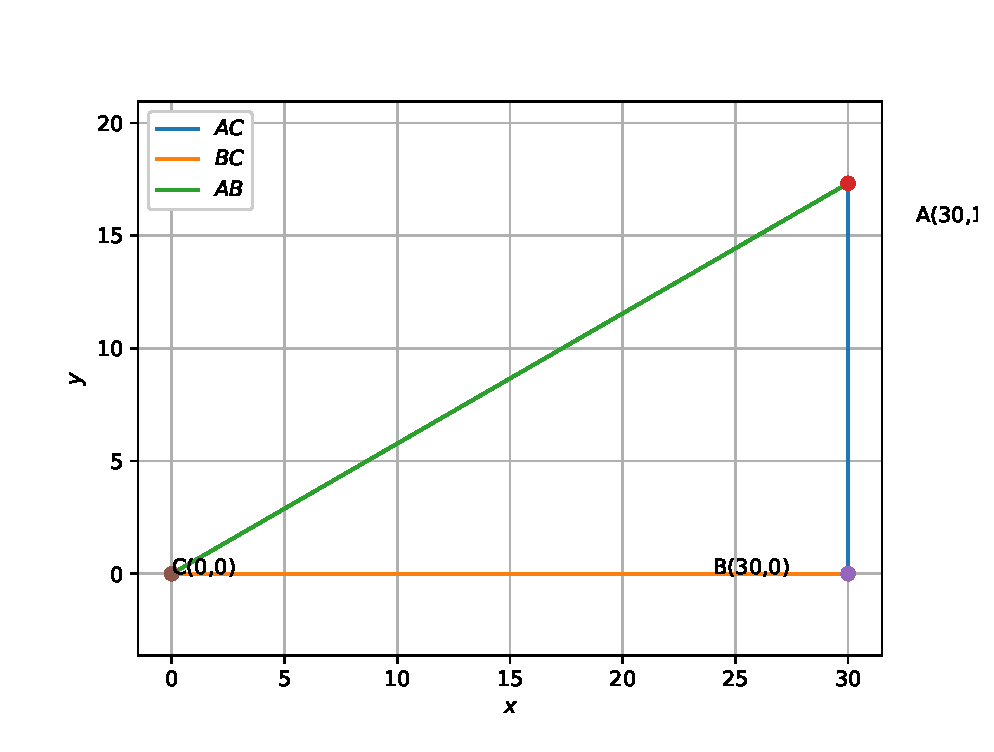
\includegraphics[width=0.8\columnwidth]{./figs/mis_ex.eps}
	\end{center}
	\caption{}
	\label{}	
\end{figure}
\end{frame}
\begin{frame}{}
\begin{figure}[!ht]
	\begin{center}
		\resizebox{0.8\columnwidth}{!}{
\begin{tikzpicture}[scale=1]

%Triangle sides
\def\a{30}
\def\c{17.34}

%Marking coordiantes
\coordinate [label=above:$A$] (A) at (\a,\c);
\coordinate [label=below:$B$] (B) at (\a,0);
\coordinate [label=left:$C$] (C) at (0,0);

%Drawing triangle ABC
\color{blue}
\draw (A) -- node[right] {$\textrm{10$\sqrt{3}$}$} (B);
\color{black}
\draw (B) -- node[below] {$\textrm{30}$} (C) -- node[above left,xshift=2mm] {$\textrm{$\sqrt{1200}$}$} (A);

%Drawing and marking angles
\tkzMarkAngle[fill=red!40,size=0.8cm,mark=](B,C,A)
\tkzMarkRightAngle[fill=blue!20,size=.3](A,B,C)
\tkzLabelAngle[pos=0.65](A,C,B)[right]{$30\degree$}

\end{tikzpicture}

}
	\end{center}
	\caption{}
	\label{}	
\end{figure}
\end{frame}
\begin{frame}
\textbf{Coordinates:}
\begin{enumerate}
\item Construct a triangle ABC which is right angled at B with a = 30, b = $10\sqrt{3}$ $\&$ C = 30$\degree$.
\item Direction vector m is equals to C-A.
\item The vertices of $\Delta$ABC are A = $\begin{pmatrix} a\\b \end{pmatrix}$, B = $\begin{pmatrix} a\\0 \end{pmatrix}$, C = $\begin{pmatrix} 0\\0 \end{pmatrix}.$ 
\end{enumerate}
\url{https://github.com/Narendrapulipati/geometry/blob/master/figs/mis_ex.tex}\\
\url{https://github.com/Narendrapulipati/geometry/blob/master/codes/mis_ex.py}
\end{frame}